\documentclass[11pt,letterpaper]{article}
\usepackage[margin=0.9in]{geometry}
\usepackage[T1]{fontenc}
\usepackage{lmodern,microtype,amsmath,amssymb,mathtools}
\usepackage{graphicx,booktabs,longtable,tabularx,array,enumitem}
\usepackage{xcolor,hyperref,fancyhdr,needspace}
\usepackage[most]{tcolorbox}
\usepackage{tikz}
\usetikzlibrary{arrows.meta,positioning,calc}
\definecolor{ink}{HTML}{223B53}
\definecolor{pale}{HTML}{F0F4F7}
\definecolor{warm}{HTML}{805A26}
\hypersetup{colorlinks=true,linkcolor=ink,urlcolor=ink,citecolor=ink,
 pdftitle={Pose Embed: Understanding and Defending the Experiment},
 pdfauthor={Pose Embed project},pdfsubject={Study guide; evidence through October 28, 2026}}
\pagestyle{fancy}\fancyhf{}
\fancyhead[L]{\small Pose Embed / Study guide}
\fancyhead[R]{\small Evidence through 28 October 2026}
\fancyfoot[C]{\thepage}
\setlength{\headheight}{15pt}
\setlength{\parindent}{0pt}
\setlength{\parskip}{0.45em}
\setlength{\emergencystretch}{2em}
\clubpenalty=10000
\widowpenalty=10000
\setlist{nosep,leftmargin=1.4em,topsep=0.4em}
\setcounter{tocdepth}{2}
\newcommand{\R}{\mathbb{R}}
\newcommand{\E}{\mathbb{E}}
\newcommand{\ind}{\mathbf{1}}
\newcommand{\relu}[1]{\left[#1\right]_+}
\newcommand{\code}[1]{\texttt{\detokenize{#1}}}
\newcommand{\src}[2]{\href{https://github.com/JJCAPPE/pose-embedding/blob/b32d50f66206b561fa34867c9274fac6ba7c287d/#1}{#2}}
\newcommand{\prepsrc}[2]{\href{https://github.com/JJCAPPE/pose-embedding/blob/5d50410b07e19a980fe3b711e63b10417b40b818/#1}{#2}}
\newcommand{\source}[1]{\par\smallskip{\small\textit{Source trail:} #1}\par}
\newtcolorbox{concept}[1]{colback=pale,colframe=ink,boxrule=0.5pt,
 arc=1pt,title=#1,fonttitle=\bfseries,left=8pt,right=8pt,top=6pt,bottom=6pt}
\newtcolorbox{caution}[1]{colback=warm!4,colframe=warm,boxrule=0.5pt,
 arc=1pt,title=#1,fonttitle=\bfseries,left=8pt,right=8pt,top=6pt,bottom=6pt}
\newcolumntype{Y}{>{\raggedright\arraybackslash}X}
\newcolumntype{P}[1]{>{\raggedright\arraybackslash}p{#1}}
\newcommand{\studycheck}[1]{\begin{concept}{Check your understanding}#1\end{concept}}
\begin{document}
\hypersetup{pageanchor=false}
\begin{titlepage}
\vspace*{1.3cm}
{\large POSE EMBED\par}
\vspace{0.8cm}
{\Huge\bfseries Understanding\\and defending\\the experiment\par}
\vspace{0.65cm}
{\Large A study guide from movement data to a fair scientific claim\par}
\vspace{1.1cm}
{\large Theory, design decisions, code provenance, and verification\par}
\vspace{0.8cm}
\begin{concept}{The question}
Does the full contextual training recipe lose less one-shot retrieval accuracy
than standard contrastive training when the query's pose information is
deliberately damaged?
\end{concept}
\vfill
This guide assumes comfortable programming, matrix algebra, multivariable
calculus, and introductory probability and statistics. It develops the
machine-learning ideas needed for this study rather than reviewing basic coding.

Prepared 30 October 2026. Scientific status is based on records through
28 October 2026. All numerical teaching examples are synthetic unless explicitly
identified as recorded project evidence. No final novel-action result exists in
the records used here.
\end{titlepage}
\pagenumbering{roman}
\hypersetup{pageanchor=true}
\begingroup
\small
\setlength{\parskip}{0pt}
\tableofcontents
\endgroup
\clearpage
\pagenumbering{arabic}
\section*{How to study this guide}
\addcontentsline{toc}{section}{How to study this guide}
The goal is to explain \emph{what is being measured, why the comparison is fair,
and what evidence permits a conclusion}. You do not need to memorize test names,
cluster job numbers, hashes, or every historical implementation detail.

Read Sections~\ref{sec:question}--\ref{sec:analysis} for the scientific account.
Section~\ref{sec:verification} explains why working software is not enough and
what has actually passed. Section~\ref{sec:explain} prepares you for questions.
The appendices contain short answers, a notation reference, and source links.

At each equation, identify the objects, their shapes, and what changes during
training. At each experimental decision, ask: \emph{what alternative explanation
does this control remove, and what uncertainty remains?}

The three companion notebooks use invented, small arrays. They illustrate
geometry and gradients, fair comparisons, and paired cluster resampling. They
are learning exercises, not an alternate research pipeline or evidence that
the real study has passed a gate.

\begin{caution}{Three different kinds of statement}
\textbf{Design:} what the locked study requires.\quad
\textbf{Evidence:} what a dated run and its verification established.\quad
\textbf{Interpretation:} what may reasonably be concluded from that evidence.

For example, three complete engineering pilots are evidence that those runs
worked under their recorded conditions. They are not the planned final
comparison, and they do not automatically validate a changed runtime.
\end{caution}

The guide uses the current frozen v3 study. The earlier 26-method, fine-tuned
v2 benchmark is preserved history, not completed work or a requirement of this
December comparison. The October 28 operational checkpoint is on a preparation
branch; its local launcher changes are not claimed to have run on the cluster.

\clearpage
\section{The question and the unit of evidence}\label{sec:question}
\subsection{Start with a concrete task}
Suppose a gallery contains one clean motion example for each of twenty actions.
A query is another motion clip. The system ranks the gallery by similarity and
returns the action of the closest example. A sitting-down query should retrieve
the sitting-down example even when some joint observations are unreliable.

This is \textbf{retrieval}: find the matching example. It is not a system that
estimates joint positions from raw video, predicts rowing force, or judges
whether an action was performed well. The input already contains estimated
joint positions. The action label provides the definition of a correct match;
it does not measure every possible meaning of biomechanical similarity.

\textbf{One-shot} describes the gallery: one labeled example for each new
action. It does not mean the model learns from one training clip. The comparison
rule is learned using thousands of clips from other actions, then applied to
actions excluded from this study's head training and model selection.

Write a motion example as $x$, its action label as $y$, and its learned
representation as $z=f(x)$. Let $\mathcal A$ be the twenty gallery action labels
and $g_a$ the reference clip for action $a$. Then
\[
 \widehat y(x)=\underset{a\in\mathcal A}{\arg\max}\;s(f(x),f(g_a)).
\]
The function $s$ is cosine similarity. Later sections derive both $f$ and $s$.
No final-test labels are used to update $f$.

\subsection{The hypothesis is deliberately narrower than ``better AI''}
There are three training recipes: standard contrastive, full contextual, and
supervised contrastive (SupCon). The one confirmatory comparison is contextual
versus standard contrastive. SupCon provides a descriptive reference.

Each trained head is evaluated on clean queries and on nine damaged-query
conditions. For a method $m$, seed $s$, and corruption condition $c$, define
\[
 d_{m,s,c}=A_{m,s,0}-A_{m,s,c},
\]
where $A$ is top-1 accuracy and $0$ denotes clean input. The main effect is
\[
 \Delta=\frac{1}{3\cdot9}\sum_{s,c}
       \bigl(d_{\mathrm{contextual},s,c}-d_{\mathrm{contrastive},s,c}\bigr).
\]
Negative $\Delta$ means the contextual recipe loses fewer accuracy points under
the declared damage mixture. A later section explains uncertainty and the
prespecified decision rule.

\begin{concept}{A smaller drop is not necessarily better damaged-input accuracy}
Invented example: standard contrastive goes from 90\% clean to 75\% damaged,
a 15-point drop. Contextual goes from 80\% to 70\%, a 10-point drop.
Then $\Delta=10-15=-5$ percentage points. Contextual degrades less, but its
damaged-input accuracy is five points worse. Both statements must be reported.
\end{concept}

The hypothesis concerns a \emph{full recipe}. Its contextual term, positive
margin, and similarity regularizer differ from the standard recipe. A positive
finding cannot identify the neighborhood term alone as the cause. The omitted
extra control limits causal attribution; it does not make the declared
recipe-to-recipe comparison meaningless.

\subsection{Why use this study design?}
Freezing an existing motion encoder makes the training comparison narrower and
less expensive than fine-tuning the whole network. Holding the head architecture,
data, duration, and tuning budget fixed makes differences easier to attribute to
the training recipes. Testing unfamiliar action classes asks whether the learned
comparison transfers beyond the action labels used for training.

Damaging only queries keeps the references unchanged. The experiment can then
measure sensitivity to the query disturbance. It does not establish performance
when both gallery and query are damaged, or robustness to arbitrary camera
failures. Those would be different experiments.

\source{\src{plan/research-plan.v3.md}{Final v3 plan, Sections 1, 3--6};
\src{docs/decisions/0004-frozen-one-shot-v3.md}{Decision 0004}.}

\section{Data: what one row actually means}\label{sec:data}
\subsection{Dataset, observations, and dependence}
The dataset family is NTU RGB+D 120,\cite{ntu} but this pipeline uses its adopted
\textbf{HRNet-derived 2D pose annotations}. The model channels are $x$ coordinate,
$y$ coordinate, and confidence. They are not $x,y,z$ ground-truth 3D positions.
``Clean'' means before this study adds damage; the pose estimates already have
their own errors.

The adopted inventory has 113,945 usable captures. Together with 535 documented
missing-skeleton exclusions, these reconcile to 114,480 nominal captures.
Reconciling the count matters because a changed input inventory could silently
change the population being compared.

A capture has metadata including setup, performer, repetition, action, and
camera. Several cameras can observe the \emph{same underlying performance}.
Thus three rows need not be three independent examples. The performance-group
key is
\[
  (\text{setup},\text{performer},\text{repetition},\text{action}),
\]
with camera deliberately omitted. This key matters twice: when excluding
near-duplicate gallery performances from primary queries, and when estimating
uncertainty.

\subsection{Split by action before learning the comparison}
The 120 action classes are partitioned into 100 auxiliary actions and twenty
novel actions. Within the auxiliary set, eighty actions train candidate heads
and twenty different actions support development evaluation.

\begin{center}
\resizebox{0.96\linewidth}{!}{%
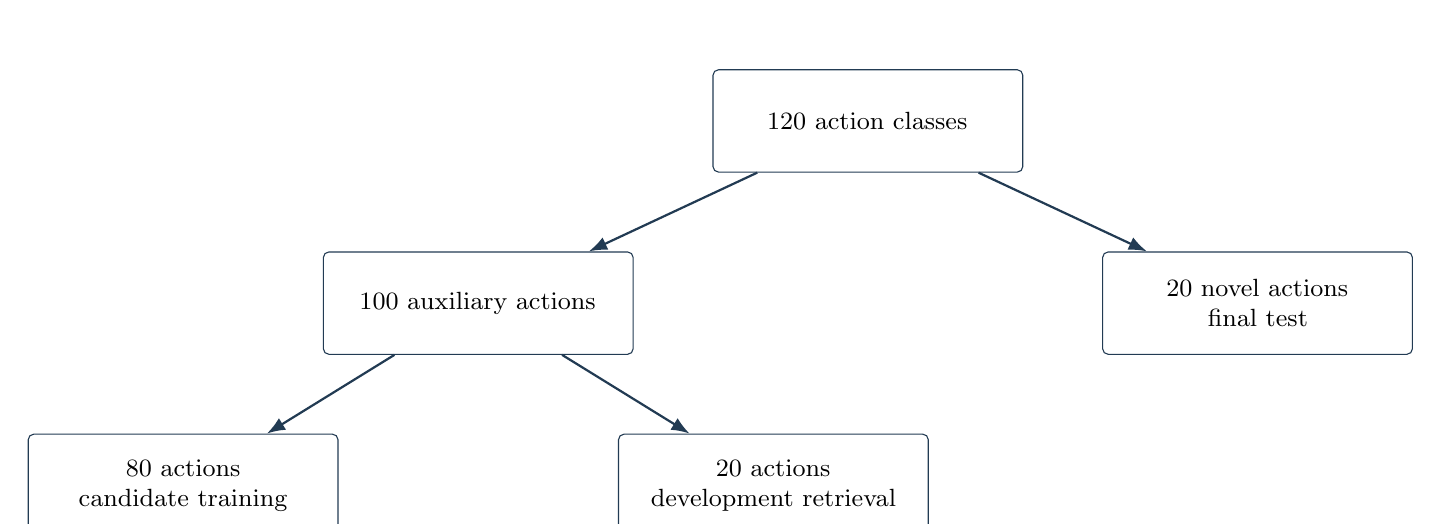
\begin{tikzpicture}[node distance=8mm,
 box/.style={draw=ink,rounded corners=2pt,align=center,text width=37mm,
 minimum height=13mm,font=\small},arrow/.style={-{Latex},thick,ink}]
\node[box] (all) {120 action classes};
\node[box,below left=10mm and 10mm of all] (aux) {100 auxiliary actions};
\node[box,below right=10mm and 10mm of all] (novel) {20 novel actions\\final test};
\node[box,below left=10mm and -2mm of aux] (train) {80 actions\\candidate training};
\node[box,below right=10mm and -2mm of aux] (dev) {20 actions\\development retrieval};
\draw[arrow] (all)--(aux);\draw[arrow] (all)--(novel);
\draw[arrow] (aux)--(train);\draw[arrow] (aux)--(dev);
\end{tikzpicture}
}
\end{center}

\begin{tabularx}{\linewidth}{@{}Y r Y@{}}
\toprule
Role & Rows & Permitted use\\\midrule
Candidate-head training & 76,013 & Learn weights using eighty actions.\\
Development-validation pool & 18,988 & Twenty held-out auxiliary actions.\\
Development gallery & 20 & One fixed reference per development action.\\
Primary development queries & 18,929 & Evaluate candidates without gallery-performance views.\\
Final-head training & 95,001 & All 100 auxiliary actions, after selecting recipes.\\
Novel gallery & 20 & Fixed official exemplars.\\
Primary novel queries & 18,884 & Confirmatory final evaluation.\\
Exact-official novel queries & 18,924 & Descriptive compatibility evaluation.\\
\bottomrule
\end{tabularx}

These rows are \emph{roles}, not disjoint quantities to add together. Final-head
training is the union of the two auxiliary pools: $76{,}013+18{,}988=95{,}001$.
Gallery and query roles are selected from their respective validation or novel
pools. The twenty novel anchors plus 18,924 official queries give 18,944 novel
rows; $95{,}001+18{,}944=113{,}945$.

After choosing one learning rate for each recipe, nine fresh final heads are
trained on all 100 auxiliary actions. Reusing the development actions at this
point is legitimate because recipe selection is finished and the novel actions
still provide the final evaluation. The final heads are not the candidate or
pilot checkpoints with new names.

\subsection{Why two query definitions?}
The exact-official query set removes the gallery exemplar itself. The primary
set also removes other camera views of that exemplar's performance. Otherwise,
the system could retrieve a simultaneously recorded version of the same event,
which is easier than recognizing another performance of the action.

The two definitions answer related but different questions. The official one
maintains benchmark comparability; the primary one reduces this specific
cross-camera dependence. Their difference is not selected after seeing scores.
Exact IDs are locked from metadata. Do not infer counts by assuming every
performance has three valid camera views.

This is an \textbf{action-disjoint} study, not a claim of performer-disjoint
generalization. People or setups can recur. ``Novel'' describes the role in
this study's head training and selection; it does not prove the pretrained
encoder has never encountered any related action in any source data.

\subsection{A manifest is part of the experimental definition}
A manifest records which sample IDs belong to a role, their order, exclusions,
and source bindings. Its hash is a compact fingerprint of those exact bytes.
Recreating a manifest independently and comparing it checks that the stated
rules lead to the same population.

This is stronger than checking a row count. Two files can each contain 18,884
rows but describe different queries. Conversely, equal hashes establish equality
of content, not that the content is scientifically correct. Both semantic
validation and identity checks are needed.

\studycheck{Why would a random split of capture rows fail to test the intended
transfer to new actions? Why is removing only the exact gallery filename
insufficient? Answers: Questions 1--2 in the answer key.}
\source{\src{plan/research-plan.v3.md}{Final v3 plan, Section 3};
\src{docs/protocol/ntu-manifest-audit.v2.md}{Adopted manifest audit};
\src{docs/protocol/input-contract-amendment.v1.md}{Input contract amendment}.}

\clearpage
\section{From joint observations to a comparison vector}\label{sec:representation}
\subsection{Follow the shapes}
One deterministically prepared example has shape
\[
 X\in\R^{2\times100\times17\times3}.
\]
The axes are person slot, sampled frame, joint, and $(x,y,\text{confidence})$.
A missing second person is represented by a padded slot. Temporal sampling
selects 100 frame positions; it is not a claim that the original recording
lasted 100 frames or that all clips had the same physical duration.

The preparation sequence is camera normalization, person tracking, conversion
from the COCO joint convention to the H36M joint convention, uniform temporal
sampling, padding, and spatial normalization. Tracking tries to keep person
slots consistent over time. Conversion produces the joint arrangement expected
by the pretrained model. Normalization removes some dependence on image position
and scale; it does not eliminate viewpoint, tracking, or pose-estimation errors.

Some converted joints combine several source joints. Their coordinates can be
averaged, but the local implementation uses the \emph{minimum} confidence of
the contributing joints. If one necessary source is absent, its derived joint
should not acquire high confidence merely because another source is visible.
This is an explicit departure from upstream confidence handling.

\begin{center}
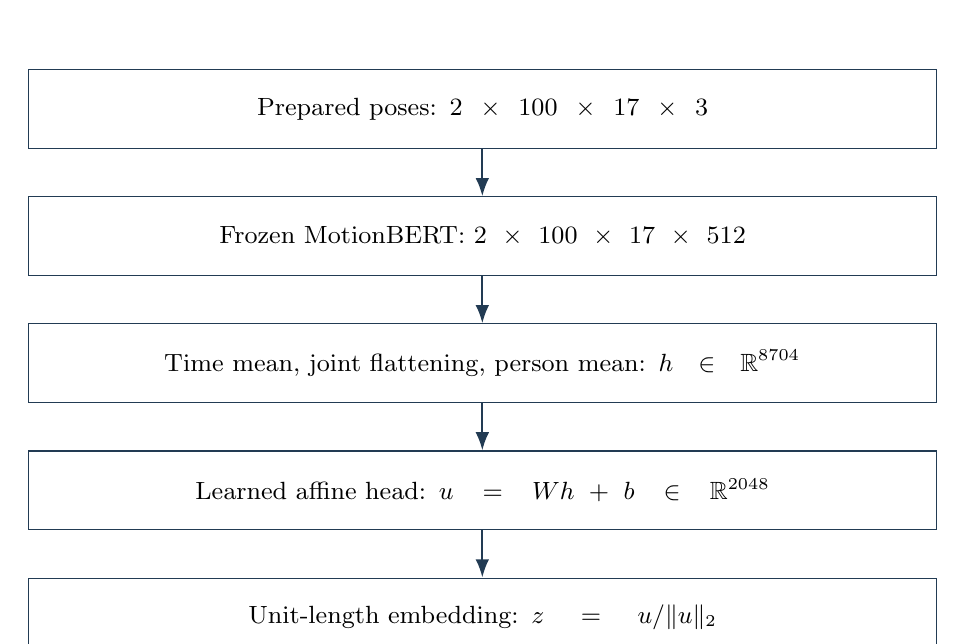
\begin{tikzpicture}[node distance=6mm,
 box/.style={draw=ink,align=center,text width=113mm,minimum height=10mm,font=\small},
 arrow/.style={-{Latex},thick,ink}]
\node[box] (x) {Prepared poses: $2\times100\times17\times3$};
\node[box,below=of x] (f) {Frozen MotionBERT: $2\times100\times17\times512$};
\node[box,below=of f] (h) {Time mean, joint flattening, person mean: $h\in\R^{8704}$};
\node[box,below=of h] (u) {Learned affine head: $u=Wh+b\in\R^{2048}$};
\node[box,below=of u] (z) {Unit-length embedding: $z=u/\lVert u\rVert_2$};
\draw[arrow] (x)--(f);\draw[arrow] (f)--(h);\draw[arrow] (h)--(u);\draw[arrow] (u)--(z);
\end{tikzpicture}
\end{center}

\subsection{What MotionBERT contributes}
A representation is a numerical description useful for a later task. Raw
coordinates describe where joints were observed. Learned features can combine
positions across joints and time so that the next stage need not learn all
motion structure from scratch.

MotionBERT was pretrained to recover motion structure from partial or noisy 2D
observations using a 3D reconstruction objective. This study reuses its generic
pretrained encoder. The adapter requests its internal representation and bypasses
its 3D output head. There is no newly estimated 3D skeleton that must be evaluated
between our input poses and retrieval vectors.\cite{motionbert}

The essential transformer operation is attention. Put a set of token features
in a matrix $H\in\R^{L\times d}$, one token per row. Learned matrices produce
\[
 Q=HW_Q,\qquad K=HW_K,\qquad V=HW_V.
\]
The query--key dot product measures which tokens should exchange information.
For each row, softmax turns scores into positive weights that sum to one:
\[
 a_{ij}=\frac{\exp(q_i^\top k_j/\sqrt{d_k})}
 {\sum_\ell\exp(q_i^\top k_\ell/\sqrt{d_k})},
 \qquad o_i=\sum_j a_{ij}v_j.
\]
The square-root factor moderates score scale as the key dimension grows.
Unlike a fixed temporal average, these weights depend on the input. Multiple
attention heads provide several learned ways to mix information, while
position information distinguishes joints and time indices.

MotionBERT's spatial attention exchanges information among joints in a frame;
temporal attention exchanges information across frames. Its two streams apply
spatial and temporal operations in opposite orders and fuse their outputs.
You need to understand this role, not reproduce every transformer layer to
explain this experiment. The pretrained implementation is imported intact.

\textbf{Frozen} and \textbf{evaluation mode} are different controls. Frozen
parameters receive no training updates. Evaluation mode selects inference
behavior for modules with training-dependent behavior, such as dropout. The
project uses both, so all recipes share a fixed feature extractor.

\subsection{Why averaging features does not discard all motion information}
Let $F_{p,t,j,:}(X)\in\R^{512}$ denote an encoder output. The pre-head vector is
\[
 h(X)=\frac12\sum_{p=1}^{2}
       \operatorname{vec}_{j}\!\left(\frac1{100}
       \sum_{t=1}^{100}F_{p,t,j,:}(X)\right)\in\R^{17\cdot512}.
\]
Here $\operatorname{vec}_{j}$ concatenates the seventeen joint feature vectors.
The mean is taken after the encoder has combined information across time. It
is therefore not equivalent to averaging raw poses before any motion processing.
It still imposes an information bottleneck: whatever the pooled representation
does not retain cannot be recovered by the head.

With a frozen encoder, $h(X)$ can be calculated once and stored in a feature
cache. This saves repeated encoder work across head-training runs. A cache is
valid only for its exact source data, preprocessing, encoder weights, code,
and relevant runtime. A damaged query needs a fresh encoder pass on the damaged
tensor; adding noise to a cached vector would be a different intervention.

\subsection{The trainable head and the geometry of retrieval}
The trained transformation is
\[
 u=Wh+b,\qquad W\in\R^{2048\times8704},\quad b\in\R^{2048},
 \qquad z=\frac{u}{\lVert u\rVert_2}.
\]
There are $2048(8704+1)=17{,}827{,}840$ trainable parameters. The architecture
is simple, but its parameter count is not tiny. The cached $h$ vectors are
\emph{not} unit-normalized; the normalization follows the learned projection.
Zero projections are an invalid numerical state to detect rather than meaningful
directions for retrieval.

For nonzero vectors $u,v$, cosine similarity is
\[
 \cos(u,v)=\frac{u^\top v}{\lVert u\rVert\lVert v\rVert}.
\]
It compares direction rather than length. Once both vectors have unit norm,
$s_{ij}=z_i^\top z_j$. Expanding a squared distance gives
\[
 \lVert z_i-z_j\rVert^2
 =z_i^\top z_i+z_j^\top z_j-2z_i^\top z_j=2-2s_{ij}.
\]
Thus sorting by largest cosine is the same as sorting by smallest squared
Euclidean distance on these unit vectors. This equivalence is why the contextual
neighborhood can be expressed using $\max(2-2s_{ij},0)$. The maximum only guards
against a tiny negative distance from floating-point arithmetic.

\begin{concept}{A two-coordinate retrieval example}
Let a query be $q=(0.8,0.6)$ and the two gallery vectors be $g_1=(1,0)$ and
$g_2=(0,1)$. All are unit vectors. Their cosine scores are $0.8$ and $0.6$,
so $g_1$ ranks first. The squared distances are $0.4$ and $0.8$, producing
the same ranking. Multiplying the unnormalized query by ten changes neither
its normalized direction nor the ranking.
\end{concept}

The output has 2,048 coordinates, not 120 class probabilities. Labels influence
the geometry during learning; an unfamiliar action can still be recognized by
comparison with its gallery exemplar. Contextual neighborhoods affect training,
but \textbf{all three recipes use the same cosine retrieval at evaluation}.
There is no contextual reranking added at query time.

\subsection{From a loss to a weight update}
A loss $L(\theta)$ assigns a penalty to the current behavior, with
$\theta=(W,b)$. Minimizing it requires a direction in parameter space.
For a small perturbation $\delta$,
\[
 L(\theta+\delta)\approx L(\theta)+\nabla L(\theta)^\top\delta.
\]
Taking $\delta=-\eta\nabla L$ lowers this local approximation when $\eta>0$.
That is the basic gradient-descent idea. It does not promise global improvement
for an arbitrarily large step, or a global optimum for this nonconvex objective.

Backpropagation is the chain rule applied through the computation. For
$z=u/\lVert u\rVert$ away from zero,
\[
 \frac{\partial z}{\partial u}
 =\frac{I-zz^\top}{\lVert u\rVert}.
\]
The factor $I-zz^\top$ removes the component parallel to $z$: changing only
magnitude does not change direction. If $g_u=\partial L/\partial u$, then
\[
 \frac{\partial L}{\partial W}=g_u h^\top,
 \qquad \frac{\partial L}{\partial b}=g_u.
\]
Batch gradients add the contributions prescribed by the loss reduction. The
encoder weights do not enter the update. Notebook 1 works through a small
normalized-head gradient numerically; its simple loss is explicitly not the
project's full training objective. This is ordinary backpropagation through
differentiable operations. The hard contextual neighborhood instead uses a
prescribed surrogate gradient, explained in the next section.

\subsection{Why AdamW, and what is fixed?}
The actual optimizer is AdamW. For gradient $g_t$, it keeps exponentially weighted
first and second moments,
\[
 m_t=\beta_1m_{t-1}+(1-\beta_1)g_t,\qquad
 v_t=\beta_2v_{t-1}+(1-\beta_2)g_t^2,
\]
and corrects their startup bias: $\widehat m_t=m_t/(1-\beta_1^t)$ and
$\widehat v_t=v_t/(1-\beta_2^t)$. The essential elementwise update is
\[
 \theta_t=(1-\eta\lambda_w)\theta_{t-1}
       -\eta\frac{\widehat m_t}{\sqrt{\widehat v_t}+\varepsilon_o}.
\]
The first term is decoupled weight decay; the second uses recent gradient
direction and scale. Weight decay is distinct from the contextual recipe's
mean-similarity regularizer, which acts on embeddings through the loss.

All recipes use $\beta_1=0.9$, $\beta_2=0.999$, $\varepsilon_o=10^{-8}$,
and $\lambda_w=10^{-4}$ on weight and bias. Learning rate is constant within
a run. There is no scheduler, dropout, extra augmentation, gradient clipping,
early stopping, or mixed precision. These are fixed controls, not assertions
that these choices are universally optimal.

\studycheck{Explain why a frozen encoder still permits learning, why the head
can recognize an action absent from its training labels, and why perturbing
cached features would change the experiment. Answers: Questions 3--4.}
\source{\src{src/pose_embed/data/motionbert.py}{Deterministic preprocessing};
\src{src/pose_embed/models/motionbert.py}{Encoder adapter};
\src{src/pose_embed/models/action_head.py}{Pooling and head};
\src{src/pose_embed/training/runner.py}{Training runner};
\href{https://github.com/Walter0807/MotionBERT/blob/705d3a95354db8bdb696b3492e47a3b5537174ff/lib/model/DSTformer.py}{Pinned DSTformer source}.}

\section{What is reused, adapted, and written for this study}\label{sec:provenance}
The research contribution is not a new pose detector or a new transformer
backbone. It is the specified transfer comparison and the controlled process
needed to interpret its result.

\begin{longtable}{@{}P{0.21\linewidth}P{0.33\linewidth}P{0.40\linewidth}@{}}
\toprule Component & Provenance & Role and boundary\\\midrule\endhead
Pose data & Existing NTU dataset and HRNet-derived pose annotations distributed
through OpenMMLab/PYSKL & Reuse the available estimates. No new HRNet training,
video collection, or native 25-joint 3D input.\\\addlinespace
MotionBERT encoder & Unchanged code imported from a pinned Apache-2.0 checkout;
verified pretrained checkpoint & Reuse the architecture and learned weights;
neither source clone nor checkpoint is committed into this repository.\\\addlinespace
Preprocessing & Minimal licensed port of MotionBERT action-data utilities & Make
sampling deterministic, preserve confidence through tracking/conversion, and
apply the declared confidence correction.\\\addlinespace
Pooling and head & Ported MotionBERT action-head semantics & Reuse time/person
pooling and projection structure; train fresh head weights for our objectives.\\\addlinespace
Contextual loss & Independently implemented from published equations, developed
from the project's teaching implementation & The authors' source repository is
reference-only because no license was discovered. It is not copied or adapted.\\\addlinespace
Contrastive and SupCon & Local implementations of the declared formulas & Make
reduction rules, margins, temperature, and single-view semantics explicit.\\\addlinespace
Optimization engine & PyTorch tensor operations, autograd, and AdamW & Reuse
numerical machinery; local code defines which parameters and batches it updates.\\\addlinespace
Training and evaluation & Local protocol-specific runners & Train on cached
auxiliary features; keep novel evaluation out of the training loop.\\\addlinespace
Experimental controls & Local manifests, sampler, corruptions, locks, provenance,
analysis, and report code & Define a reproducible experiment rather than inherit
benchmark defaults.\\\bottomrule
\end{longtable}

\subsection{Why not reuse the upstream one-shot training loop?}
That loop evaluates novel classes during training. Our study requires those
outcomes to remain unavailable until training, selection, and the final lock
are complete. Reusing the encoder is compatible with this requirement; reusing
that evaluation schedule is not. The local head-training loop is a necessary
change in scientific procedure, not a claim that upstream code is defective.

\subsection{Two kinds of provenance}
\textbf{Intellectual provenance} identifies whose method, data, and code are
being used, along with the permitted reuse and attribution. \textbf{Execution
provenance} identifies the exact source revision, checkpoint, input IDs,
configuration, and runtime that produced an artifact. A result needs both.

Historical v2 contains other methods and upstream sources, but those are not all
used in this v3 comparison. The current study does not need a tour of every
preserved benchmark implementation. Nor does a source repository being publicly
viewable establish permission to copy its code; the project's source manifest
and notices record that boundary.

\source{\src{third_party/upstreams.toml}{Pinned upstream manifest};
\src{THIRD_PARTY_NOTICES.md}{Third-party notices};
\src{docs/protocol/ntu-input-source-research.md}{Pose-source investigation};
\src{docs/protocol/motionbert-adapter-gate.md}{Adapter reuse boundary};
\src{docs/protocol/contextual-v3-source-notes.md}{Contextual source and equation notes}.}

\clearpage
\section{The three training recipes, from first principles}\label{sec:losses}
\subsection{What a training batch tells the model}
For a batch of $n$ normalized embeddings, form the similarity matrix
$S=ZZ^\top$, where row $i$ of $Z$ is $z_i^\top$. Let
\[
 y_{ij}=\ind[\text{action}_i=\text{action}_j].
\]
A \emph{positive pair} has the same action label; a \emph{negative pair} has
different labels. These names describe supervision, not good or bad examples.
The losses encourage a geometry consistent with those labels.

Each physical batch has eight action classes and four examples per class:
$P=8$, $K=4$, $n=PK=32$. Each anchor has three nonself positives and twenty-eight
negatives. The full matrix contains 96 directed positive pairs and 896 directed
negative pairs, excluding self-pairs. A directed pair counts $(i,j)$ separately
from $(j,i)$; the declared reductions handle that consistently.

Why not draw thirty-two arbitrary examples? An unbalanced random batch may have
too few same-label examples to provide the required positive relations. The
balanced sampler controls that issue and supplies the local population in which
contextual neighborhoods are defined.

\subsection{Standard contrastive: enforce similarity margins}
We want positive similarities to be sufficiently high and negative similarities
to be sufficiently low. Define a hinge $[a]_+=\max(a,0)$:
\[
 h^+_{ij}=[m_+-s_{ij}]_+,
 \qquad h^-_{ij}=[s_{ij}-m_-]_+.
\]
For the standard recipe, $m_+=0.9$ and $m_-=0.6$. A positive pair with
similarity $0.7$ receives a penalty $0.2$. A negative pair with similarity $0.7$
receives a penalty $0.1$. Positive similarity above $0.9$ and negative similarity
below $0.6$ produce no hinge penalty. The interval between the margins is an
intentional gap, not a probability threshold for an action classifier.

Define the strictly active sets
\[
 \mathcal A_+=\{(i,j):i\ne j,\ y_{ij}=1,\ h^+_{ij}>0\},\quad
 \mathcal A_-=\{(i,j):y_{ij}=0,\ h^-_{ij}>0\}.
\]
Then
\[
 L_{\mathrm{contrast}}=
 \frac{\sum_{(i,j)\in\mathcal A_+}h^+_{ij}}{|\mathcal A_+|}
 +\frac{\sum_{(i,j)\in\mathcal A_-}h^-_{ij}}{|\mathcal A_-|},
\]
where an empty active set contributes zero.

This detail is consequential: these are separate means over \emph{violations},
not one mean over all pairs. An abundance of already-satisfied negatives does
not dilute the remaining negative violations. The hinges are not squared.
Away from boundaries and changes in the active set, each active positive gives
derivative $-1/|\mathcal A_+|$ with respect to its similarity; each active
negative gives $+1/|\mathcal A_-|$. Through the chain rule these gradients change
$W,b$ so the relevant similarities move toward their margins.

\subsection{Context: ask how examples relate to the rest of the batch}
Direct similarity examines a pair. Contextual similarity also examines its
relations to other examples. Two noisy instances can be more convincingly
related if their neighborhoods agree. That is a motivation, not a guarantee:
bad neighborhoods can also reinforce bad relationships.

The current implementation has five steps: find nearby examples, measure shared
neighbors and non-neighbors, keep that agreement local, expand using reciprocal
neighbors, then make the score symmetric. The final score is trained to match
the same-action indicator $y_{ij}$. It is not trained to imitate the current
cosine matrix; doing that would change the target of the learning problem.

The following equations specify the local implementation. Their source trail
is the protocol and independently written local code; the contextual paper
provides the method's intellectual origin.\cite{contextual}

\subsubsection*{Step 1: define a neighborhood}
Compute squared unit-vector distances and a binary membership matrix:
\[
 d_{ij}=\max(2-2s_{ij},0),\qquad
 N_{ij}=\ind[d_{ij}\le d_{i,(k)}+\epsilon].
\]
$d_{i,(k)}$ is the $k$th smallest distance in row $i$. Here $k=4$ and
$\epsilon=0.05$. \textbf{Self is included} in the ordering. The tolerance
admits points just beyond the $k$th distance, so the neighborhood may contain
more than four examples, especially with ties.

The symbol $k$ is a neighbor rank used to set the distance cutoff; $K$ is
examples per class. Both equal
four in the fixed recipe, but their conceptual roles differ. Labels do not
choose the neighbors. Current embedding distances do.

\subsubsection*{Step 2: compare neighborhood membership}
For row $i$, set
\[
 a_i=\max\left(\sum_\ell N_{i\ell},1\right),\qquad
 b_i=\max\left(\sum_\ell(1-N_{i\ell}),1\right).
\]
The first-stage score is
\[
 A_{ij}=\frac12\left(
  \frac{\sum_\ell N_{i\ell}N_{j\ell}}{a_i}
 +\frac{\sum_\ell(1-N_{i\ell})(1-N_{j\ell})}{b_i}
 \right)N_{ij}.
\]
The numerators count shared neighbors and shared non-neighbors. The row
denominators turn them into fractions relative to $i$. Multiplication by
$N_{ij}$ restricts the score to pairs already in $i$'s neighborhood. The clamp
keeps an empty complement from creating division by zero; it is a declared
local finite convention.

\begin{concept}{Work one neighborhood calculation by hand}
In an invented six-example batch, let $i=1$ have neighbors $\{1,2,3,4\}$ and
$j=2$ have neighbors $\{1,2,3,5\}$. They share three of $i$'s four neighbors.
Their non-neighbor sets are $\{5,6\}$ and $\{4,6\}$, sharing one of two.
Because $N_{12}=1$,
\[
 A_{12}=\tfrac12(3/4+1/2)=0.625.
\]
This is only the first-stage score, not the final contextual similarity or
the cosine similarity. With unequal row sizes, $A_{ij}$ need not equal $A_{ji}$.
\end{concept}

\subsubsection*{Step 3: reciprocal expansion and symmetry}
Construct another neighborhood $N^{1/2}$ using the $k/2$ threshold and the
same tolerance. A reciprocal relation requires both directions:
\[
 R_{i\ell}=N^{1/2}_{i\ell}N^{1/2}_{\ell i}.
\]
Use those reciprocal neighbors to average first-stage rows, then symmetrize:
\[
 B_{ij}=\frac{\sum_\ell R_{i\ell}A_{\ell j}}
 {\max(\sum_\ell R_{i\ell},1)},\qquad
 C_{ij}=\frac{B_{ij}+B_{ji}}2.
\]
This incorporates the local relationship profiles of mutually close examples.
Symmetry gives a common score for the pair regardless of direction.

\subsubsection*{Step 4: fit action-label agreement}
The contextual penalty is
\[
 L_{\mathrm{context}}=\frac1{n^2}\sum_{i\ne j}(C_{ij}-y_{ij})^2.
\]
It asks contextual similarity to approach one for same-action pairs and zero
for different-action pairs. Self terms are omitted, but the denominator remains
$n^2$, not $n(n-1)$. Even a small reduction change can alter gradient scale and
therefore the relative weight of the objectives.

\subsection{How can a hard neighborhood comparison have a gradient?}
An indicator is locally constant almost everywhere and discontinuous at its
boundary. Its ordinary derivative cannot provide useful smooth updates for
moving points between neighborhoods. The recipe deliberately uses a
\textbf{straight-through estimator} (STE): perform the hard comparison in the
forward pass, but prescribe a surrogate derivative in the backward pass.

For the comparison $H(x,y)=\ind[x\ge y]$, the implemented rule assigns
\[
 \frac{\widetilde{\partial}H}{\partial x}=\alpha,\qquad
 \frac{\widetilde{\partial}H}{\partial y}=-\alpha,\qquad \alpha=10.
\]
The tilde emphasizes that this is a chosen backward rule, not the ordinary
derivative of the hard function. In the neighborhood expression, $x=-d_{ij}
+\epsilon$ and $y=-d_{i,(k)}$.

The $k$th-distance thresholds and first-stage counts are \emph{detached}: they
retain their forward values but are treated as constants during differentiation.
The reciprocal denominator in $B$ is \emph{not} detached. It participates in the
backward calculation. These choices are part of the fixed method, not details
that an optimizer can infer from a prose description.

\begin{caution}{What a derivative check can and cannot establish}
For a smooth head calculation, finite differences can check an analytic
gradient. For this hard comparison, a finite difference will usually see zero
while the prescribed STE returns a nonzero value. That disagreement is expected.
Verification must check the declared surrogate backward rule independently;
it must not claim the rule is the true derivative of the hard forward function.
\end{caution}

\subsection{The full contextual recipe includes two more terms}
The recipe also contains the margin contrastive loss and a mean-similarity
regularizer:
\[
 L_{\mathrm{reg}}=
 \left(\frac1{n^2}\sum_{i,j}s_{ij}-0.25\right)^2,
 \qquad
 L_{\mathrm{full}}=0.4L_{\mathrm{context}}
                  +0.6L_{\mathrm{contrast}}+0.1L_{\mathrm{reg}}.
\]
The regularizer includes diagonal entries. Its target controls average batch
similarity; it is not an action probability or a guarantee against collapse.
The contrastive term here uses $m_+=0.75$ and $m_-=0.6$, whereas the standalone
contrastive arm uses $m_+=0.9$.

That means a contextual win could arise from the combined effects of neighborhood
structure, a different margin, and regularization. Separating their contributions
would require matched ablations, including the omitted control. This study
instead compares the two complete declared recipes within its available scope.

The fixed values transfer a published recipe into a pose study. They were not
established as optimal pose hyperparameters. Do not substitute defaults from
an older teaching class or historical protocol for the explicit v3 configuration.

\subsection{SupCon: rank all positive examples against the batch}
Let $P(i)=\{p\ne i:y_{ip}=1\}$. SupCon assigns a softmax distribution over
every nonself example and penalizes the log probability of each positive:
\[
 L_{\mathrm{SupCon}}=-\frac1n\sum_i\frac1{|P(i)|}
   \sum_{p\in P(i)}\log
   \frac{\exp(s_{ip}/\tau)}{\sum_{a\ne i}\exp(s_{ia}/\tau)},
 \qquad \tau=0.07.
\]
For one anchor, every positive should rank well relative to all alternatives.
The denominator includes other positives as well as negatives; self is excluded.
Using the log converts a product-like probability objective into a sum and
strongly penalizes a positive assigned very small probability.

Temperature $\tau$ sets sensitivity to score gaps. Two alternatives whose
similarities differ by $0.14$ have softmax weight ratio
$\exp(0.14/0.07)=\exp(2)\approx7.39$. A smaller temperature makes the same
gap matter more. This does not make the value a calibrated probability that
an arbitrary final query has a particular action.

The study uses a single-view adaptation: no second augmented view and no extra
temperature multiplier. SupCon is supervised because action labels define
positives. It is not being used as a label-free pretraining method here.
In the ideal limit of zero probability on negatives, equal allocation among
three positives gives per-anchor loss $\log 3$ rather than zero. Raw loss values from different
recipes are therefore not a common accuracy scale.\cite{supcon}

\subsection{What fairness does and does not require}
All recipes receive the same architecture, data, batch plans, initialization
within a seed, training duration, and learning-rate grid. They are allowed to
use different objective formulas because that is the treatment being compared.
Equal tuning opportunities do not mean equal floating-point operation counts,
nor that each method reaches its own global optimum.

\begin{tabularx}{\linewidth}{@{}Y Y Y@{}}
\toprule Recipe & Main training signal & Interpretation boundary\\\midrule
Contrastive & Fix positive/negative margin violations & A specified baseline,
not every possible contrastive method.\\
Full contextual & Neighborhood agreement, contrastive margins, mean similarity
& Effects belong to the full recipe.\\
SupCon & Positive log probabilities against the batch & Descriptive reference;
no additional superiority test.\\\bottomrule
\end{tabularx}

\studycheck{Why is gradient accumulation from four batches of eight examples
not equivalent to one physical batch of thirty-two? Why would a contextual
win not isolate the neighborhood term? Why should loss magnitudes not be ranked
across recipes? Answers: Questions 5--7.}
\source{\src{src/pose_embed/losses/pairwise.py}{Contrastive and SupCon formulas};
\src{src/pose_embed/losses/contextual.py}{Local contextual implementation};
\src{docs/protocol/contextual-v3-source-notes.md}{Equation and recipe decisions};
\src{configs/protocol.v3.yaml}{Locked v3 settings}.}

\clearpage
\section{How the comparison is made fair}\label{sec:design}
\subsection{Specify the experiment before looking for a winner}
A machine-learning result combines choices about data, representation, objective,
optimization, model selection, and evaluation. If those choices are changed
after seeing a preferred method's outcomes, apparent improvement can reflect
the selection process rather than a reliable advantage.

The v3 protocol fixes the hypothesis, action splits, gallery, recipes, duration,
tuning grid, corruption conditions, analysis, and reporting rules before
selection and final-test access. This is a \emph{prespecified} comparison. A
hash-bound configuration makes the exact specification checkable; it does not
replace a scientific explanation of why the choices are appropriate.

\begin{longtable}{@{}P{0.28\linewidth}P{0.32\linewidth}P{0.34\linewidth}@{}}
\toprule Controlled choice & What stays the same & Alternative explanation reduced\\\midrule\endhead
Representation & Encoder, checkpoint, preprocessing, head structure & A different
backbone or input pipeline caused the difference.\\\addlinespace
Optimization exposure & Twenty epochs, physical $8\times4$ batches & One recipe
received more updates or different within-batch information.\\\addlinespace
Initialization and order & Exact initial weights and ordered batches within seed
& A favorable starting state or example order caused the difference.\\\addlinespace
Tuning budget & Three rates, three seeds per rate, same ranking rule & More search
opportunities gave one method an advantage.\\\addlinespace
Evaluation input & Same gallery, queries, and per-example damage & Methods were
evaluated on different problems.\\\addlinespace
Claim rule & One primary effect and fixed interval construction & A favorable
metric, subset, or threshold was chosen afterward.\\\bottomrule
\end{longtable}

These controls improve \textbf{internal validity}: whether the observed
difference answers the declared comparison. \textbf{External validity} asks
whether it transfers to other datasets, people, actions, cameras, or damage
mechanisms. Internal controls alone cannot establish that broader claim.

\subsection{Pairing is more than using the same seed}
Let $A_s$ and $B_s$ denote outcomes from two methods under a paired condition.
For their difference,
\[
 \operatorname{Var}(A_s-B_s)
 =\operatorname{Var}(A_s)+\operatorname{Var}(B_s)
  -2\operatorname{Cov}(A_s,B_s).
\]
Shared difficulty can induce positive covariance, making the difference less
variable than an unpaired comparison. Pairing is useful even when that variance
reduction is not guaranteed: it prevents known input differences from becoming
uncontrolled method differences.

A seed initializes a pseudorandom generator. It does not prove two execution
paths consumed random values in the same order or used the same arithmetic.
The project therefore stores and verifies exact starting-state and batch-plan
identities. Seeds 7, 17, and 29 give three paired training realizations.
They produce three separate heads per method, \emph{not an ensemble}.

An epoch is defined as $\lceil N/32\rceil$ balanced batches. For candidate
training, $\lceil76{,}013/32\rceil=2{,}376$ updates per epoch and 47,520 over
twenty epochs. Class and example queues are shuffled at the epoch start and
cycled within it. This is a balanced update budget, not a guarantee that every
row is visited exactly once per epoch.

Gradient accumulation cannot replace the physical batch: relationships between
examples in different microbatches never exist in either microbatch's similarity
matrix. Adding their gradients cannot retroactively construct the missing
neighbors, positives, or softmax alternatives.

\subsection{Pilots, model selection, and final training are separate}
\textbf{Engineering pilots} answer whether the implementation can complete the
specified training and produce valid numerical artifacts. There is one pilot
per recipe, at seed 7 and learning rate $3\times10^{-4}$, for twenty epochs.
Checkpoints at epochs 5, 10, 15, and 20 plus epoch-zero diagnostics expose the
training behavior. Their accuracy does not select a learning rate or a winning
method. A pilot that happens to share a candidate's settings is still ineligible
for selection.

\textbf{Model selection} chooses the learning rate separately for each recipe:
\[
 3\text{ recipes}\times3\text{ rates}\times3\text{ seeds}=27\text{ fresh runs},
 \qquad\eta\in\{10^{-4},3\times10^{-4},10^{-3}\}.
\]
Rank candidates using unrounded mean epoch-20 clean development top-1 accuracy
over all three seeds. Resolve exact ties with mean MRR, then lower learning rate.
The best checkpoint is not selected across epochs. Corrupted development scores
are not tuning criteria. If an endpoint learning rate wins, the grid is not
expanded after the fact.

\textbf{Final training} starts nine fresh heads: three recipes at their selected
rates, each with three paired seeds, using all 95,001 auxiliary examples. All nine
must finish and be locked before novel evaluation. A final run is not a pilot
continued for longer, a selected checkpoint reused unchanged, or a seed chosen
because it looked favorable.

\begin{concept}{What a failed run means}
A candidate needs all three valid seeds; averaging only its two successful
seeds changes the comparison. Preserve failures and their causes. An allowed
infrastructure retry repeats identical inputs in a new attempt; it is not a
chance to draw a better seed. Numerical failure and poor accuracy are different:
poor but valid accuracy is a scientific outcome, while nonfinite computation
invalidates the affected evidence.
\end{concept}

The fixed twenty-epoch duration avoids choosing a favorable stopping point.
It does not claim that every method has converged or received its ideal budget.
The fair statement is equal declared training and selection opportunities,
with cost and limitations reported.

\subsection{Why keep the final test closed?}
Repeatedly looking at test results can influence human choices even if no
test gradient is computed. Picking margins, a split, a corruption, or a headline
after observing novel outcomes would use the test for development.

The study therefore progresses through separate authorizations: auxiliary
engineering, selection, final-head locking, and only then the single novel
evaluation campaign. A dataset-level opening record spans historical and current
versions so a new output folder cannot silently reset the holdout's history.
After opening, scientific training and selection for this study/source remain
closed. An error discovered afterward must be preserved and reported; a corrected
analysis cannot silently replace the confirmatory result.

There is a historical packaging nuance. The original aggregate loader
deserialized all annotations before selecting auxiliary records. The evidence
supports no novel retrieval preprocessing, embedding, visualization, scoring,
or tuning access; it does not support the stronger claim that no novel bytes
were ever deserialized. The newer auxiliary package separates authorized inputs
from novel processing. State the actual access boundary, not a cleaner-sounding
history.

\source{\src{plan/research-plan.v3.md}{Plan, Sections 4 and 9};
\src{src/pose_embed/training/sampler.py}{Balanced sampler};
\src{docs/protocol/protocol-v3.md}{Fixed recipes, selection, and staged authorization}.}

\section{Designing a controlled disturbance}\label{sec:corruption}
\subsection{Where the intervention occurs}
Write preprocessing as $P$, frozen encoding and pooling as $F$, and the learned
head as $H_m$. Clean retrieval uses $H_m(F(P(x)))$. A damaged query uses
\[
 z_{m,c}=H_m\bigl(F(T_c(P(x)))\bigr),
\]
where $T_c$ changes the prepared pose tensor. The gallery remains clean.
This location is part of the scientific question: the study perturbs pose
observations, not rendered pixels, model weights, training labels, or cached
embedding coordinates.

Each family starts from its own clean tensor. Damage families are not combined.
After damage, there is no clipping, recentering, normalization, interpolation,
or frame deletion that could alter the declared intervention.

\begin{tabularx}{\linewidth}{@{}P{0.20\linewidth}P{0.24\linewidth}Y@{}}
\toprule Family & Three strengths & What changes and what stays fixed\\\midrule
Coordinate jitter & 1\%, 2.5\%, 5\% of torso scale & Gaussian offsets to observed
$x,y$ coordinates; confidence and missing observations unchanged.\\\addlinespace
Joint masking & 3, 6, 8 joints & Zero complete trajectories, including confidence,
using nested prefixes of one anatomically grouped ordering.\\\addlinespace
Frame masking & 10, 25, 40 of 100 frames & Zero a contiguous nested interval across
people, joints, and channels; retain all 100 time slots.\\\bottomrule
\end{tabularx}

\subsection{Scale jitter to the body, not arbitrary pixels}
For observed joint coordinates, the intervention has the form
\[
 x'_{p,t,j,:2}=x_{p,t,j,:2}+\sigma\,r(x)\,\eta_{p,t,j},
 \qquad\eta_{p,t,j}\sim\mathcal N(0,I_2).
\]
$\sigma$ is a fixed severity and $r(x)$ is the clean sample's lower-median
positive finite torso scale. Thus the noise standard deviation is expressed
relative to body size. A sample without usable torso geometry uses one fixed
fallback: the lower median of valid sample-level scales from the eighty-action
training set. It is measured and frozen before the relevant runs, not estimated
from final-test poses or tuned to produce convenient damage.

The same Gaussian field is reused at all three severities, multiplied by the
corresponding scale. That keeps the disturbance direction fixed while changing
its magnitude. Missing or padded observations remain missing rather than being
turned into plausible new joints.

\subsection{Nested severity and shared randomness}
Per-example randomness is determined by the sample identity and corruption
family, not by method, training seed, or severity. Joint masks use nested
prefixes; frame intervals are coupled so larger intervals contain smaller ones.
Therefore, when severity increases, it strengthens the same intervention.
It does not accidentally replace it with an unrelated easier random pattern.

The same damaged tensor is evaluated for every recipe and seed. A comparison
then measures different responses to the same disturbance. It does not compare
one model's fortunate noise draw with another model's unfortunate draw.

\subsection{Validate the intervention before interpreting performance}
A declared ``40-frame mask'' should zero the intended forty slots without
shortening the sequence. Jitter should preserve confidence and scale with the
declared body measure. The geometry panel checks interpretable examples and edge
cases; full-query damage summaries establish what happened across the evaluation
population, including fallback use and zero-damage cases.

That evidence is a manipulation check: did $T_c$ do what the experiment says?
It does not establish that contextual training handles the damage better.
The October development damage audit passed its recorded execution/damage
checks, but later runtime-dependent evidence still requires regeneration.

These are controlled tensor stress tests. Real occlusion may cause a pose
estimator to hallucinate confident joints rather than set them to zero; real
frame loss may have another temporal pattern. MotionBERT was already pretrained
with masking/noise. The present experiment studies the incremental effect of
head-training recipes on that shared encoder.

\studycheck{Why exclude severity from the random seed? Why measure fallback
scale only from training poses? Why is masking input coordinates not equivalent
to simulating a camera occlusion? Answers: Questions 8--9.}
\source{\src{docs/protocol/protocol-v3.md}{Corruption conventions};
\src{src/pose_embed/corruptions/pose.py}{Corruption operators};
\src{src/pose_embed/corruptions/fallback.py}{Training-only fallback};
\src{docs/protocol/week-5-execution.md}{Recorded development damage audit}.}

\section{From retrieval ranks to a defensible conclusion}\label{sec:analysis}
\subsection{Compute ranks first, then metrics}
Let $r_q$ be the rank of the one correct gallery exemplar for query $q$.
With a fixed gallery order to break exact cosine ties,
\[
 \mathrm{Top1}=\frac1Q\sum_q\ind[r_q=1],\qquad
 \mathrm{R@5}=\frac1Q\sum_q\ind[r_q\le5],\qquad
 \mathrm{MRR}=\frac1Q\sum_q\frac1{r_q}.
\]
For invented ranks $(1,2,7,1)$, Top-1 is $2/4=0.5$, R@5 is $3/4=0.75$, and
MRR is $(1+1/2+1/7+1)/4\approx0.661$. Top-1 asks whether the immediate answer
is correct. R@5 asks whether the correct answer is in a short list. MRR rewards
moving the correct answer closer to the top even when it is not first.

With exactly one relevant gallery item, average precision per query is $1/r_q$,
so mAP equals MRR. Reporting both would not add independent evidence.

The complete final report has
\[
 3\text{ recipes}\times3\text{ seeds}\times10\text{ conditions}
 \times2\text{ query definitions}=180\text{ cells}.
\]
The ten conditions are clean plus nine corruptions. These are 180 reporting
cells, not 180 independent experiments: the same heads, examples, and damage
draws recur across them. The two query sets also overlap heavily.

\subsection{Derive the primary effect at the query level}
Let $a_{m,s,c,q}\in\{0,1\}$ indicate a correct top-1 prediction. For each
primary query, compute
\[
 e_q=\frac1{27}\sum_{s,c}
 \left[(a_{C,s,0,q}-a_{C,s,c,q})
       -(a_{B,s,0,q}-a_{B,s,c,q})\right],
\]
where $C$ is contextual and $B$ is standard contrastive. Then
\[
 \Delta=\frac1Q\sum_q e_q.
\]
This equals the earlier difference of mean accuracy drops because sums can be
reordered. A query that becomes correct after corruption contributes a negative
drop; the definition does not clip improvements to zero.

Queries have equal weight within each cell. The three seeds and nine corruption
conditions have equal weight in the declared mixture. This does not imply the
nine conditions are equally common in the world. It defines the specific stress
mixture whose average effect is being tested.

An algebraic check connects the headline to absolute performance:
\[
 \Delta=(A_{C,\mathrm{clean}}-A_{B,\mathrm{clean}})
        -(\overline A_{C,\mathrm{corrupt}}-\overline A_{B,\mathrm{corrupt}}).
\]
Always report all three quantities. An accuracy difference of $0.03$ is
\emph{three percentage points}, not a three-percent relative increase. It
corresponds descriptively to thirty additional correct matches per thousand
queries under the specified mixture.

\subsection{Why ordinary row resampling would be misleading}
The observed $\Delta$ is a number for this fixed collection of trained heads
and examples. To characterize sampling variation within that setting, the
protocol uses a bootstrap: repeatedly resample the observed units with
replacement and recompute the statistic.

The resampling unit must reflect dependence. If several cameras recorded the
same performance, resampling each view independently treats correlated evidence
as if it came from separate events. The project instead samples entire
performance groups, preserving all available camera views together.

The declared procedure is:
\begin{enumerate}
\item Within each of the twenty fixed actions, identify the performance groups.
\item Sample that action's original number of groups with replacement. A group
selected twice contributes all its queries twice.
\item Use the same sampled groups across all methods, seeds, and conditions.
\item Sum their per-query effects and divide by the total sampled query count.
\item Repeat 10,000 times with the fixed generator seed, then take the 2.5th and
97.5th percentiles using the prescribed linear quantile convention.
\end{enumerate}
Actions and training seeds are \emph{not} resampled. This is not a bootstrap
over all possible tasks or all possible training runs.

\subsection{Unequal camera counts change the denominator}
Suppose one sampled performance group contains one query with effect $+1$ and
another contains three queries each with effect $-1$. The query-weighted mean is
\[
 \frac{1-1-1-1}{4}=-0.5.
\]
The mean of the two group means would be $(1+(-1))/2=0$, which answers a
different question. Groups are resampled together to respect dependence, but
queries retain their declared weighting. Resampling is not permission to change
the estimand, meaning the exact quantity we intend to estimate.

Because groups can have different numbers of views, each bootstrap draw can
contain a different query count. The denominator must be recomputed. Actions
remain fixed strata, but their queries are not forced to have equal action
weights. Notebook 3 demonstrates this with small arrays.

\subsection{What the interval means and the rule for the claim}
The 95\% percentile interval describes uncertainty under the chosen resampling
scheme. The 95\% is a nominal repeated-sampling coverage target under its
assumptions, not a 95\% probability that the contextual recipe is superior.
The single confirmatory statement is supported only if its \emph{upper}
bound is below zero. An interval spanning zero is inconclusive for that claim;
it does not prove equivalence or that the true effect is exactly zero.

\begin{tabularx}{\linewidth}{@{}Y Y@{}}
\toprule Observed pattern & Permitted interpretation\\\midrule
Upper bound below zero & Evidence of less contextual degradation under the
declared mixture. Check absolute corrupted accuracy separately.\\\addlinespace
Interval includes zero & Insufficient evidence for the declared smaller-drop
claim; no equivalence conclusion.\\\addlinespace
Lower bound above zero & Evidence points toward more contextual degradation
under the declared mixture.\\\bottomrule
\end{tabularx}

\begin{caution}{The interval's scope is conditional}
It conditions on the trained heads, the three fixed seeds, fixed actions,
gallery anchors, query definitions, and realized synthetic corruptions. It
assumes performance groups are exchangeable within an action for this resampling
purpose. Repeated performances from one person can still be dependent.

It does not quantify uncertainty over arbitrary people, new action classes,
different reference clips, unrestricted training seeds, or real camera failures.
Ten thousand bootstrap draws do not create ten thousand independent models.
\end{caution}

Three seeds expose some training variation but do not justify broad population
claims about random initializations. Every seed and condition is reported.
SupCon, exact-official results, and per-cell comparisons remain descriptive;
there are no additional unplanned superiority tests selected from favorable
rows of the 180-cell table.

\subsection{Sensitivity without changing the retrieval problem}
Leave-one-action-out analysis asks whether one action strongly determines the
reported effect. Remove that action's \emph{queries}, retaining the original
gallery and original ranks. If the gallery item were also removed, the remaining
queries would face fewer alternatives, changing the retrieval problem itself.
The ranges and sign changes are descriptive checks, not new confirmatory tests.

Report effect size, clean accuracy, absolute corrupted accuracy, per-seed and
per-condition results, cost, and failures together. A null or adverse contextual
result is successful research if the valid declared experiment is completed.
A blocked experiment with no final comparison is an honest operational outcome,
but it is not a null scientific result.

\studycheck{Why resample whole performance groups but still weight individual
queries? What does an interval crossing zero establish? Why do the three seeds
not become 10,000 seeds through bootstrapping? Answers: Questions 10--12.}
\source{\src{plan/research-plan.v3.md}{Locked analysis, Section 6};
\src{docs/protocol/protocol-v3.md}{Analysis conventions};
\src{docs/results/README.md}{Reproducible result/report contract}.}

\clearpage
\section{Verification: what each check actually establishes}\label{sec:verification}
\subsection{A chain of evidence, not a count of passing tests}
For a final claim to be useful, the implementation must compute the intended
quantity, use the intended inputs, preserve the comparison, and produce records
that can be checked independently. A large software test suite supports that
work, but its size is not a measure of scientific completion.

\begin{longtable}{@{}P{0.24\linewidth}P{0.35\linewidth}P{0.35\linewidth}@{}}
\toprule Question & Evidence that addresses it & What it does not establish\\\midrule\endhead
Are the equations implemented correctly? & Independent hand calculations of
forward values and the declared backward rules, including edge cases & That the
method works on real movements.\\\addlinespace
Does the learning path work? & A deliberately learnable synthetic problem with
healthy gradients and correct self-excluded retrieval & Good generalization or
real-data superiority.\\\addlinespace
Are the intended examples used? & Independently regenerated manifests, source
identity, overlap/exclusion checks & Independence of every observation.\\\addlinespace
Does the adapter preserve intended encoder behavior? & Local and upstream
encoder outputs on the same prepared input arrays & Byte-identical upstream
preprocessing where the local confidence rule intentionally differs.\\\addlinespace
Does an execution repeat? & Fresh-process initialization, geometry, and full-cache
repeats under the bound runtime & Correctness merely from repeating the same
error, or equality across arbitrary hardware.\\\addlinespace
Was the intervention applied? & Fixed-panel geometry and complete-query damage
summaries & Better robustness of any learned recipe.\\\addlinespace
Can results be reconstructed? & Independent projection, ranking, metric, and
report replay from bound records & Permission to reinterpret the locked claim.\\\addlinespace
Can the whole study finish? & Measured end-to-end costs, retained storage, job
windows, queue allowance, and researcher availability & Feasibility inferred
from fast training alone.\\\bottomrule
\end{longtable}

\subsection{Independent checks must be capable of disagreeing}
Calling the same production function twice can establish repeatability, but
both calls share its possible bug. A mathematical reference should derive a
small result independently, with enough simplicity to inspect manually.
For the contextual loss, both the forward formula and prescribed STE backward
rule need such evidence. A second implementation copied line for line would
not provide the same independence.

Likewise, a training process writing ``complete'' is not independent proof that
the checkpoint, inputs, and scores agree. A separate validation process checks
the retained outputs and their dependencies. A clean process also prevents an
unrecorded in-memory state from supplying missing information.

Real pilots check finite loss, gradients, and parameters, nonzero projections,
unit-vector normalization, adequate embedding variation, complete update counts,
paired initialization/batches, and measured cost. The collapse check asks whether
every example has become essentially the same vector; it does not certify that
the remaining variation is useful. There is no real-data accuracy floor that
forces the experiment to produce a favorable result.

\subsection{The reproducibility problem encountered here}
Floating-point operations round their results. Reordering sums, choosing a
different vectorized kernel, or changing the numerical runtime can change bits
even when the source expression is unchanged. A fixed random seed governs the
random-number sequence; it does not fix every arithmetic path or transformation
of those random numbers.

This project encountered both starting-weight reconstruction mismatches and
small geometry differences across execution environments. In the geometry case,
clean arrays and sample identities matched, while some derived torso scales
and jitter arrays differed. Exact repeatability within each environment did not
establish equality between them. Several diagnostics narrowed possibilities,
but the complete historical numerical cause was not established.

The authorized response was to select and record one prospective runtime,
require exact fresh-process repeatability and pairing within it, and preserve
differences from older outputs. That is an explicit change in the acceptance
requirement. It is not a claim that the old and new numbers were equal after all.

A later cluster kernel update failed the frozen-runtime startup check before
scientific training began. Such a startup failure is evidence that the runtime
binding changed, not evidence that the model produced incorrect numbers on the
new kernel. The new profile was authorized for verification, but compatibility
had to be measured rather than assumed.

\subsection{Immutable evidence and the scope of a correction}
An artifact is retained with its source, input, configuration, and runtime
bindings. A corrected release writes new artifacts with explicit predecessor
links instead of overwriting the failed attempt. This preserves the distinction
between what originally happened and what a later correction established.

The relevant software-engineering idea is dependency-aware invalidation. A
changed scientific input or implementation invalidates evidence depending on
it. It need not invalidate an unrelated unchanged manifest, but old numerical
outputs cannot be relabeled as new-runtime results without the required check.
The protocol determines which dependencies and acceptance evidence matter.

Changes are recorded with a reason and their effect on scientific settings.
The runtime amendments arose from observed reproducibility and execution
problems, with earlier development outputs already in existence. They were not
claimed to predate all development scores, and final novel outcomes remained
unavailable. The algorithms, action IDs, corruption definitions, training
duration, and claim rule stayed fixed.

\subsection{Verification itself has a cost}
The study discovered that nested validation repeatedly recomputed the same
expensive numerical checks. Under the measured old execution path, one repeated
component alone forecast over 122 hours against the old execution plan's shared
48-hour maximum-job check. That was a forecast from measured component time and call counts, not an
observed 122-hour run.

The authorized optimization reuses a successful numerical verification only
inside one guarded command, after rehashing its complete bound contents and
matching the validator settings and identities. A changed dependency prevents
reuse. Independent commands begin without inherited proof. Authorization,
dataset-opening state, resources, and other dynamic checks remain fresh.

This differs from simply skipping expensive checks: the question is whether the
\emph{identical deterministic proposition} has already been established in the
current command. The design still requires independent recertification and new
measurements of total cost.

Storage feasibility also includes retained attempts, checkpoints, feature
caches, projections, logs, temporary peaks, and a reserve. The declared rule is
\[
 \min(\text{filesystem free},\text{quota remaining})
 \ge 200\cdot2^{30}+1.25\cdot\text{remaining peak bytes}.
\]
Free disk space outside the account's quota is not usable capacity. Nor is
deleting failed scientific evidence an acceptable way to make the forecast fit.
Time forecasts similarly need the complete workflow, queue/setup allowances,
and researcher effort, not just the head-training loop.

\source{\src{docs/decisions/0006-v3-execution-completion-amendment.md}{Execution-completion amendment};
\src{docs/decisions/0007-safe-validation-reuse-and-stage-capacity.md}{Validation reuse and capacity};
\src{docs/decisions/0008-runtime-baseline.md}{Prospective runtime decision};
\src{docs/decisions/0009-updated-kernel-baseline.md}{Updated-kernel decision}.}

\section{Decisions and progress through the evidence cutoff}\label{sec:history}
\subsection{The decisions that explain the current experiment}
\begin{longtable}{@{}P{0.19\linewidth}P{0.37\linewidth}P{0.38\linewidth}@{}}
\toprule Decision & Reason & Consequence for the claim or process\\\midrule\endhead
Choose one-shot motion retrieval & Make movement comparison testable on an
existing dataset with unfamiliar action labels & Evaluate matching to one clean
example per novel action; do not claim a rowing-quality system.\\\addlinespace
Adopt a verified pose input contract & Available HRNet-derived annotations and
documented missing captures differed from initial assumptions & Bind the actual
source inventory and regenerate exact manifests.\\\addlinespace
Freeze MotionBERT and narrow to three recipes (29 Sep) & Bound the December
question and resource requirements & Compare head-training recipes; preserve
the broader fine-tuned v2 benchmark as unfinished historical scope.\\\addlinespace
Use primary and official query sets & Synchronized views can duplicate the
gallery performance & Primary excludes all such views; official-compatible
results remain descriptive.\\\addlinespace
Fix duration, pairing, grid, and claim rule & Limit unequal opportunity and
outcome-driven choices & Twenty epochs, three paired seeds, 27 selection runs,
nine final heads, one confirmatory effect.\\\addlinespace
Omit the extra regularizer control & Keep the December study bounded before
new selection outcomes & A result supports the full recipe, not the isolated
neighborhood mechanism.\\\addlinespace
Complete and rehearse the full path (9 Oct) & Successful pilots did not establish
that authorization through report generation worked & Successor releases and
fresh affected evidence before selection.\\\addlinespace
Permit guarded verification reuse (12 Oct) & Measured repeated validation exceeded
an execution limit & Preserve checks while avoiding duplicate numerical work
within an identical guarded command.\\\addlinespace
Adopt one prospective runtime (19 Oct) & Historical cross-environment equality
was not established & Keep exact within-runtime repeatability; record historical
differences honestly.\\\addlinespace
Revalidate after kernel update (25 Oct) & The observed runtime no longer matched
the accepted profile & Authorize a new profile, preserve source/settings, require
fresh affected evidence.\\\bottomrule
\end{longtable}

\subsection{What has actually been completed}
The early work established the literature basis, prospectus, dataset/access
arrangements, verified input inventory, deterministic split manifests, and
adapter implementation. September extraction established encoder agreement on
the same prepared arrays and two complete, matching 95,001-row feature passes.
Those remain historical evidence for their recorded release.

On October 8, Week 4 closed with fresh v3 caches and all three complete
twenty-epoch engineering pilots. The two full extraction passes matched exactly,
and independent checks accepted the outputs. Each pilot had 47,520 updates with
paired initial weights and batches. These are substantial execution milestones,
but the pilot scores are ineligible for selecting a winner.

October successor work completed execution/report rehearsal and the historical
full-query damage audit. The audit checked nine corruption conditions across
18,929 development queries each. Later work accepted a prospective CPU baseline,
its repeatable initialization and geometry, a synthetic GPU prerequisite, and
five caches under the then-frozen profile. The subsequent kernel change means
those records do not automatically satisfy the new-profile requirements.

The project also has a public tracker, research journal, explanatory pose
visualizations, and report/poster drafts with results explicitly pending.
Those help communicate and retain the work; they are not additional scientific
evidence of recipe superiority.

\subsection{What remains incomplete}
At the October 28 checkpoint, Week 5 remains open and cluster jobs are held
while adequate usable storage is pending. The local launcher correction and
conditional remaining-work schedule are prepared. No new-profile acceptance
or final comparison is inferred from that preparation.

The next scientific prerequisites are accepted new-runtime repeatability,
affected caches and paired pilots, development corruption/retrieval replay,
and a measured full-workload capacity decision. Only after admission can the
27 selection runs proceed, followed by nine final heads, final locks, and the
novel evaluation campaign. Selection, final training, and novel opening remain
closed in the latest record.

The original October 18 admission deadline was missed. November 29 final locks,
December 6 computation, and December 7--18 analysis/delivery remain recorded
targets; the guide does not claim the remaining schedule has been demonstrated
feasible. Live capacity was not remeasured while preparing this guide.

\begin{concept}{The accurate status sentence}
The study design and software have passed substantial engineering checks,
including historical full pilots and damage audits. The latest runtime still
needs accepted regeneration, and storage is blocking the next cluster work.
There is no final evidence yet that contextual training is better, equivalent,
or worse on the declared novel-action comparison.
\end{concept}

\source{\src{docs/protocol/week-3-scc-execution.md}{September execution evidence};
\src{docs/protocol/week-4-execution.md}{Week 4 closure};
\src{docs/protocol/week-5-execution.md}{October accepted history and kernel/storage blocker};
\prepsrc{docs/protocol/week-5-execution.md}{October 28 checkpoint};
\prepsrc{docs/protocol/week-6-handoff.md}{Conditional remaining-work calendar}.}

\clearpage
\section{Prepare to explain and defend the work}\label{sec:explain}
\subsection{A short explanation you can adapt}
\begin{concept}{About one minute}
I am testing whether a particular way of training movement representations
makes matching human actions less sensitive to damaged pose information.
At evaluation, the system gets one clean example of each unfamiliar action
and must match other clips to those examples.

I reuse a pretrained MotionBERT encoder and keep it fixed. I train the same
linear comparison head with three recipes. The main comparison is the full
contextual recipe against standard contrastive training. Both use paired
starting weights, batches, training duration, and tuning opportunities.

I damage only the query poses, using fixed strengths of coordinate noise,
missing joints, and missing frames. The primary quantity is the difference
in clean-to-damaged accuracy drops, while absolute accuracy is reported too.

Historical pilots and input checks have passed. Current work is blocked on
storage and new-runtime verification. The final comparison has not run, so I
am not claiming that the contextual recipe wins.
\end{concept}

Say this in your own words. The structure matters more than memorizing it:
question, input/output, controlled comparison, measurement, current evidence.

\subsection{A five-minute technical explanation}
\begin{enumerate}
\item \textbf{Define the task.} A sequence of estimated 2D joint positions enters
a frozen encoder, then a learned head. The output is a unit vector used for
nearest-gallery retrieval. One-shot refers to one exemplar per novel action.
\item \textbf{Define the treatment.} Compare training recipes on the same head.
The contextual recipe includes neighborhoods, a changed margin, and a regularizer;
it is not an isolated neighborhood ablation.
\item \textbf{Explain the split and tuning.} Eighty actions train candidates;
twenty other auxiliary actions select rates using clean development retrieval.
Nine fresh final heads use all 100 auxiliary actions. Twenty novel actions
remain outside selection and training.
\item \textbf{Explain the intervention.} Three damage families at three fixed
strengths act after preprocessing and before encoding. Damage is paired across
methods and nested across severities; gallery examples remain clean.
\item \textbf{Explain the statistic.} Compare clean-to-corrupt Top-1 drops,
averaged over three fixed seeds and nine conditions. Resample whole performance
groups within actions to preserve camera-view dependence. State the interval's
conditional scope and show absolute accuracy beside the drop.
\item \textbf{Separate evidence from intent.} Describe completed historical
pilots and damage checks, then the current runtime/storage prerequisite. End
with what must happen before a final claim is possible.
\end{enumerate}

\subsection{Questions someone should be able to ask you}
\textbf{Why expect contextual learning to help?}
Relations to neighboring examples may provide useful information beyond a
pair's direct similarity. That is a plausible mechanism motivating the study.
Image-domain findings do not establish robustness to noisy pose queries; this
experiment tests that transfer rather than assuming it.

\textbf{What exactly is original here?}
The backbone, pose dataset, and published objective ideas are reused. The project
specifies and implements a controlled pose-retrieval comparison, its local
adaptations, corruption design, protected evaluation, and verification/reporting
process. It is not claiming to invent MotionBERT or contextual loss.

\textbf{Why is a linear head enough?}
The nonlinear encoder already supplies rich motion features. A common affine
head limits architectural variation while still learning a different geometry.
This is a deliberate comparison setting, not proof that a nonlinear head could
not perform better. Its approximately 17.8 million parameters also mean that
``linear'' should not be confused with negligible capacity.

\textbf{Does fixed training make the comparison perfectly fair?}
It makes the stated budget and controls comparable. It does not guarantee
equal computational cost, convergence, optimal hyperparameters, or equal
compatibility with every representation. The result is conditional on these
declared recipes and settings.

\textbf{Why not choose the best pilot or early checkpoint?}
Those outputs are engineering diagnostics. Reusing them for selection or choosing
an attractive epoch would give an extra, unplanned search opportunity and change
the fixed-duration procedure. The declared fresh selection runs have one rule.

\textbf{Why keep both official and stricter query sets?}
The official set enables comparison with the established benchmark convention.
The primary set removes other cameras' views of the gallery performance,
reducing a specific shortcut. Their distinct roles are fixed before results.

\textbf{Could the model learn who the person is?}
Action-disjoint splits do not remove all person or setup dependence. Shared
people, acquisition conditions, and representation biases remain limitations.
The study is not a separate test of generalization to unseen people.

\textbf{Why are three seeds not enough for a universal claim?}
They show three fixed training realizations and allow paired comparisons.
The primary bootstrap does not resample them and cannot infer performance over
all possible training randomness. Per-seed results show how consistent this
small set is without disguising its limited scope.

\textbf{What would count as success if contextual loses?}
A valid, complete, reproducible comparison with an honest contrary result.
Scientific success is answering the specified question. Failing to complete
the comparison because of capacity is a blocked study, not evidence of no effect.

\textbf{Why has verification taken so much work?}
The experiment needs more than a model that trains. Source/input identity,
exact pairing, damaged-input validity, runtime repeatability, and independently
reconstructible results determine whether the final comparison is interpretable.
The project also learned that those checks must be included in capacity planning.

\textbf{What cannot you claim yet?}
No final recipe ranking, novel-action robustness effect, or completed empirical
comparison. Successful pilots establish their execution; report drafts and a
working tracker do not supply missing final results.

\subsection{Draw these three things without looking}
\begin{enumerate}
\item The shape pipeline: $2\times100\times17\times3$ poses to frozen features,
8,704 pooled values, a learned 2,048-dimensional unit vector, and gallery ranking.
\item The action split: eighty candidate-training actions, twenty development
actions, all 100 used only after selection for fresh final training, and twenty
separate novel actions for final evaluation.
\item A two-row result table containing clean accuracy, corrupted accuracy,
and drop. Construct a case where contextual degrades less but has worse
corrupted accuracy, then explain why both facts belong in the report.
\end{enumerate}

\subsection{Use the notebooks to test understanding}
\begin{tabularx}{\linewidth}{@{}P{0.11\linewidth}Y Y@{}}
\toprule Lab & Concept & What you should explain afterward\\\midrule
01 & Cosine geometry and a normalized-head gradient & Why direction determines
ranking; how changing $W$ changes it; what finite differences verify.\\\addlinespace
02 & Splits, leakage, pairing, and equal selection budgets & Why repeated views
and unequal tuning opportunities can distort a comparison.\\\addlinespace
03 & Degradation and paired cluster bootstrap & Why smaller drop can coexist
with worse accuracy; why the sampled query count is the denominator.\\\bottomrule
\end{tabularx}

All examples are invented. Do not report their scores as project results.
Notebook 1 simplifies the training objective to make differentiation visible;
it does not implement or validate the contextual STE. Notebook 3 implements the
analysis logic on a tiny synthetic population, not the locked real-data campaign.

\appendix
\clearpage
\section{Answers to the study checks}
\begin{enumerate}[label=\textbf{\arabic*.},leftmargin=2em]
\item \textbf{Random row splits.} They can put the same action classes in
training and evaluation, testing new clips of familiar actions rather than
transfer to unfamiliar actions. They can also separate synchronized views of
one performance across roles.
\item \textbf{Gallery exclusion.} A different camera file can still depict the
same event as the gallery example. The primary set excludes the underlying
performance group, not only one filename.
\item \textbf{Learning with a frozen encoder.} The encoder's output stays fixed,
but the head's $W,b$ change how those features map into comparison directions.
A novel action does not need a learned output-class coordinate: it supplies a
gallery exemplar and is recognized by similarity to it.
\item \textbf{Cache perturbation.} A pose corruption is transformed nonlinearly
by the encoder. In general $F(T(X))$ is not equivalent to adding noise to $F(X)$.
The intervention location is therefore part of the hypothesis.
\item \textbf{Physical batch.} Pairwise similarities, contextual neighbors, and
SupCon denominators depend on the examples simultaneously present. Summing
gradients from separate smaller batches omits cross-microbatch relations.
\item \textbf{Full recipe.} Contextual and standard contrastive differ in the
neighborhood term, positive margin, and similarity regularizer. A matched
ablation would be needed to isolate one component's causal contribution.
\item \textbf{Loss magnitudes.} The formulas, reductions, coefficients, and
attainable minima differ. Compare retrieval under the common evaluation,
not which method reports the smallest numerical training loss.
\item \textbf{Shared severity randomness.} Reuse of the underlying noise field
or nested mask makes a stronger level a controlled strengthening of the same
damage. Unrelated draws could obscure the effect of increasing severity.
\item \textbf{Fallback and realism.} A training-only fallback avoids estimating
preprocessing parameters from held-out poses. Synthetic zero masks and Gaussian
noise do not reproduce every output a real pose estimator produces under camera
occlusion, so they support a narrower robustness claim.
\item \textbf{Groups versus query weights.} Groups preserve dependence during
resampling; query weights preserve the chosen statistic. Equal weighting of
unequal-sized group means would change the quantity being estimated.
\item \textbf{Interval crossing zero.} The data do not support the prespecified
smaller-drop claim at that rule. This is neither proof of equality nor an
estimate that the probability of no effect is 95\%.
\item \textbf{Bootstrap draws and seeds.} Repeatedly resampling performance
groups recombines evidence from the same three heads per method. It creates no
new independent training realizations or uncertainty over unobserved seeds.
\end{enumerate}

\section{Notation and essential terms}
\begin{longtable}{@{}P{0.25\linewidth}P{0.68\linewidth}@{}}
\toprule Symbol or term & Meaning here\\\midrule\endhead
$X$ & Prepared pose tensor for one capture.\\
$h\in\R^{8704}$ & Frozen, pooled, unnormalized pre-head feature vector.\\
$W,b$ & Trainable affine head weights and bias.\\
$u\in\R^{2048}$; $z$ & Head output before normalization; its unit-length direction.\\
$s_{ij}$; $d_{ij}$ & Cosine similarity; squared unit-vector distance.\\
$y_{ij}$ & Indicator that two training examples have the same action label.\\
$P,K,n$ & Classes per batch, examples per class, and physical batch size.\\
$k,\epsilon,\alpha$ & Contextual neighbor rank, membership tolerance, and
surrogate-gradient factor.\\
$\tau$; $\eta$ & SupCon temperature; optimizer learning rate.\\
$A_{m,s,c}$; $d_{m,s,c}$ & Top-1 accuracy and clean-to-corrupt drop; this $d$ has
method/seed/condition indices, unlike pairwise distance $d_{ij}$.\\
$\Delta$ & Contextual drop minus contrastive drop, averaged over fixed seeds
and corruptions. Negative favors less contextual degradation.\\
Gallery; query & Labeled reference examples; the example to be matched.\\
Embedding & A learned numerical representation used for comparison.\\
Epoch & The prescribed number of balanced updates, not necessarily one visit
to each row.\\
Hyperparameter & A setting chosen outside gradient updates, such as learning
rate; distinct from learned weights.\\
Leakage & Information from an evaluation role influences development or makes
the evaluation easier in a way the claimed design excludes.\\
Estimand & The exact quantity the experiment intends to estimate.\\
Bootstrap & Recompute a statistic over repeated resamples of the declared units.\\
Provenance & The source, input, configuration, and runtime identities connecting
an output to the execution that produced it.\\
Gate & An explicit requirement and its acceptance evidence before later work
is eligible.\\\bottomrule
\end{longtable}

\section{Source map and evidence boundaries}\label{sec:sources}
The linked repository sources are pinned to commit
\code{b32d50f66206b561fa34867c9274fac6ba7c287d}, the main-branch record through
October 25, unless marked as the October 28 preparation record at
\code{5d50410b07e19a980fe3b711e63b10417b40b818}. This keeps the account traceable
even if a live branch later changes. The guide is explanatory documentation;
the canonical protocol and authorized amendments control execution.

\begin{longtable}{@{}P{0.29\linewidth}P{0.65\linewidth}@{}}
\toprule Read this for & Primary project source\\\midrule\endhead
Scientific question and rules & \src{plan/research-plan.v3.md}{Final v3 plan}
and \src{docs/protocol/protocol-v3.md}{protocol v3}.\\\addlinespace
Machine-readable settings & \src{configs/protocol.v3.yaml}{Protocol template}
and \href{https://github.com/JJCAPPE/pose-embedding/tree/b32d50f66206b561fa34867c9274fac6ba7c287d/configs/experiments/v3}{27 candidate configurations}. A template is
not an executed or resolved design lock.\\\addlinespace
Method equations and adaptation & \src{docs/protocol/contextual-v3-source-notes.md}{Contextual source notes},
\src{src/pose_embed/losses/contextual.py}{contextual loss}, and
\src{src/pose_embed/losses/pairwise.py}{pairwise losses}.\\\addlinespace
Reuse and preprocessing & \src{third_party/upstreams.toml}{Upstream manifest},
\src{THIRD_PARTY_NOTICES.md}{notices}, and
\src{docs/protocol/motionbert-adapter-gate.md}{adapter acceptance}.\\\addlinespace
Why the scope changed & \src{docs/decisions/0004-frozen-one-shot-v3.md}{Decision 0004};
\src{docs/decisions/0006-v3-execution-completion-amendment.md}{0006},
\src{docs/decisions/0007-safe-validation-reuse-and-stage-capacity.md}{0007},
\src{docs/decisions/0008-runtime-baseline.md}{0008}, and
\src{docs/decisions/0009-updated-kernel-baseline.md}{0009}.\\\addlinespace
Accepted history and current state & \src{docs/protocol/week-4-execution.md}{Week 4},
\src{docs/protocol/week-5-execution.md}{Week 5 through October 25}, and
\prepsrc{docs/protocol/week-5-execution.md}{October 28 current checkpoint}.\\\bottomrule
\end{longtable}

The October 28 schedule's opening prose overstates the October 25 filesystem
failure. The numerical Week 5 record shows quota below the requirement while
filesystem free space exceeded it; usable space was still insufficient because
the minimum governs. This guide uses the numerical record and states the
storage blocker without treating an old observation as live capacity.

The intended prerequisites are general calculus, linear algebra, elementary
probability/statistics, and strong programming. No transcript, grades, student
identifier, or private academic record is included. Figures are schematic and
notebook data are synthetic. No licensed pose array, learned checkpoint,
participant record, or private operational log is included.

\begin{thebibliography}{9}
\addcontentsline{toc}{section}{Research origins}
\bibitem{ntu} J. Liu et al. \emph{NTU RGB+D 120: A Large-Scale Benchmark for
3D Human Activity Understanding}. IEEE TPAMI, 2020.
\href{https://arxiv.org/abs/1905.04757}{Authors' paper};
\href{https://rose1.ntu.edu.sg/dataset/actionRecognition/}{Official dataset}.
The local input contract separately identifies the adopted HRNet-derived 2D
annotations; the dataset's title does not make our input coordinates 3D.
\bibitem{motionbert} W. Zhu et al. \emph{MotionBERT: A Unified Perspective on
Learning Human Motion Representations}. ICCV, 2023.
\href{https://openaccess.thecvf.com/content/ICCV2023/html/Zhu_MotionBERT_A_Unified_Perspective_on_Learning_Human_Motion_Representations_ICCV_2023_paper.html}{Official paper and supplement}.
Read for the encoder's original purpose; our frozen-head comparison is a
different experiment from its downstream fine-tuning results.
\bibitem{contextual} C. Liao, T. Tsiligkaridis, and B. Kulis.
\emph{Supervised Metric Learning to Rank for Retrieval via Contextual Similarity
Optimization}. ICML, 2023.
\href{https://proceedings.mlr.press/v202/liao23b.html}{Paper and appendix}.
Read for the contextual objective's origin. The local source notes resolve
equation/backward conventions and document pose-study adaptations.
\bibitem{supcon} P. Khosla et al. \emph{Supervised Contrastive Learning}.
NeurIPS, 2020.
\href{https://papers.nips.cc/paper/2020/hash/d89a66c7c80a29b1bdbab0f2a1a94af8-Abstract.html}{Official paper}.
Read for label-based contrastive learning; this study fixes a single-view variant.
\end{thebibliography}

\end{document}
